\chapter{Bağımlılaştırma ve eşgüdüm} \label{ch:subord-coord-tr}

\epigraph{If I were a cinnamon peeler\\
I would ride your bed\\
and leave the yellow bark dust\\
on your pillow.}{Michael Ondaatje, \enquote{The Cinnamon Peeler}}

\begin{tblsframedsymbol}{Öğrenme hedefleri}{bulb}
\begin{itemize}[noitemsep, leftmargin=*]
    \item Bağımlılaştırma ile eşgüdüm arasındaki farkı ayırt etmek: biri hiyerarşik bağımlılık kurar, öteki eş statülü ögeleri birleştirir.
    \item Karmaşık cümlelerde matris, ana ve bağımlı tümceleri belirleyip çözümlemek.
    \item İçerik, karşılaştırma ve ilgi tümceleri gibi farklı bağımlı tümce türlerini tanımak.
    \item Bağımlılaştırıcıların ve eşgüdümleyicilerin baş değil, yapısal işaretleyici olarak çalıştığını anlamak.
    \item Öbek ve tümce eşgüdümü dahil olmak üzere eşgüdümlü yapıları çözümlemek.
    \item Karmaşık cümlelerde yapısal ilişkileri belirlemek için tanılayıcı testleri kullanmak.
    \item Bağımlılaştırma ile eşgüdümün metinsel bağdaşıklık kurmak için birlikte nasıl çalıştığını görmek.
    \item Bu yapıların sözdizimsel farkındalık geliştirme açısından öğretim değerini kavramak.
\end{itemize}
\end{tblsframedsymbol}

\section{Giriş}

Dil, yalnızca tek tek fikirleri değil, fikirler arasındaki ilişkileri de ifade etmemizi sağlar. Bunu yapmanın iki temel yolu vardır: \term{bağımlılaştırma} (\term{subordination}) ve \term{eşgüdüm} (\term{coordination}). Her birinin ayrı bir işi vardır: bağımlılaştırma bağımlılık hiyerarşileri kurar; eşgüdüm ise eş statülü ögeleri birleştirir.

Aynı temel fikirleri bağlamanın şu üç yolunu düşünün:

\ea \label{ex:intro-tr}
    \ea \gll Kim left. Pat came.\\
        Kim ayrıl-GEÇMİŞ Pat gel-GEÇMİŞ\\
    \glt `Kim ayrıldı. Pat geldi.' [ayrı]
    \ex \gll The fact {\ob}that Kim left{\cb} enabled Pat's arrival.\\
        DEF olgu BAĞ Kim ayrıl-GEÇMİŞ mümkün-kıl-GEÇMİŞ Pat-GEN geliş-POSS\\
    \glt `Kim'in ayrılması Pat'in gelişini mümkün kıldı.' [bağımlı]
    \ex \gll Kim left and Pat came.\\
        Kim ayrıl-GEÇMİŞ ve Pat gel-GEÇMİŞ\\
    \glt `Kim ayrıldı ve Pat geldi.' [eşgüdümlü]
    \z
\z
(\ref{ex:intro-tr}a)'da iki bağımsız bildirim var. (b)'de \mention{that Kim left} daha büyük bir yapının içine yerleşmiştir: özne içindeki bir tamlayıcı olarak iş görür. (c)'de ise iki tümce aynı düzeye konmuştur: eş konumdadırlar ve yalnızca \mention{and} ile bağlanmışlardır.

Hiyerarşi ile eşitlik arasındaki bu karşıtlık dilbilgisinin derinlerine iner. Bir tümceyi başka bir tümceye bağımlılaştırdığımızda bir bağımlılık ilişkisi kurarız: bir tümce, ötekindeki bir ögenin tamlayıcısı ya da niteleyicisi olur. Ögeleri eşgüdümlediğimizde ise, başka bakımlardan farklı olsalar bile, yapı içinde eş statülü olduklarını söyleriz.

Bu farklı ilişkiler için kullandığımız araçlar sayıca azdır. Bağımlılık ilişkileri için \mention{that} ve \mention{whether} gibi sözcükler, eşitlik ilişkileri içinse \mention{and}, \mention{or} ve \mention{but} gibi sözcükler kullanılır. Ama bu küçük sözcükler, basit parçalardan karmaşık anlamlar kurmamızı, fikirlerin birbirine nasıl bağlandığını göstermemizi ve okuru uzun akıl yürütme zincirleri boyunca yönlendirmemizi sağlar. Bu ögeler baş gibi davranmaz; dilbilgisel ilişkiyi gösterir.

Bu bölümde bu iki sistemin hem ayrı ayrı hem de birlikte nasıl çalıştığını göreceğiz. Bağımlılaştırmanın bir düşünceyi başka bir düşüncenin içine yerleştirerek anlam katmanları kurduğunu inceleyeceğiz. Eşgüdümün ise yapısal yalınlığı korurken karmaşık fikirler kurmamızı nasıl sağladığını göreceğiz. Son olarak, iki sistemin birbirini nasıl tamamladığını, yani aklımıza gelebilecek hemen her fikir ilişkisini ifade etmek için bize nasıl esneklik verdiğini göstereceğiz.

\section{Bağımlılaştırma}\label{sec:subordination-tr}

İletişim kurarken fikirler arasında karmaşık ilişkiler ifade etmemiz sık sık gerekir. Bazen bir fikir başka bir fikre bağlıdır; bazen bir düşünce başka bir düşünceyi nitelemek ya da açıklamak için kullanılır. Bağımlılaştırma tam burada devreye girer. \term{Bağımlılaştırma}, bir tümceyi başka bir yapının içinde \term{bağımlı öge} (\term{dependent}) yapma sürecidir.

\term{Bağımlı tümce} (\term{subordinate clause}) içeren tümceye \term{matris tümce} (\term{matrix clause}) denir. Kendisini içine alan bir matris tümce bulunmayan tümce ise \term{ana tümce} (\term{main clause}) olarak adlandırılır. Aşağıdaki örnek, bir tümcenin hem ana tümce hem de matris tümce olabileceğini gösterir.

\ea \label{ex:sub-basic-tr}
    \ea \gll Kim left early.\\
        Kim ayrıl-GEÇMİŞ erken\\
    \glt `Kim erken ayrıldı.' [ana]
    \ex \gll She thinks {[}that Kim left early{]}.\\
        o düşün-ŞİMDİ {[}BAĞ Kim ayrıl-GEÇMİŞ erken{]}\\
    \glt `Kim'in erken ayrıldığını düşünüyor.' [bağımlı]
    \ex \gll {[}She thinks that Kim left early{]}.\\
        {[}o düşün-ŞİMDİ BAĞ Kim ayrıl-GEÇMİŞ erken{]}\\
    \glt `Kim'in erken ayrıldığını düşünüyor.' [ana/matris]
    \z
\z
(\ref{ex:sub-basic-tr}a) basit bir ana tümcedir. (b)'de köşeli parantezlerle gösterilen aynı tümce bağımlı hâle gelmiştir; artık (c)'deki matris tümcenin içinde bir bağımlı ögedir. (c)'deki matris tümce aynı zamanda ana tümcedir.

Bu örüntü genişletilebilir. (\ref{ex:sub-basic2-tr})'de, (\ref{ex:sub-basic-tr}b)'deki yapı ana tümce olmaktan çıkıp bağımlı tümceye dönüşmüştür; ama \mention{that Kim left} için matris tümce olmayı sürdürür. Yani bir tümce yalnızca hem ana hem matris değil, hem bağımlı hem matris de olabilir.

\ea\label{ex:sub-basic2-tr}
\gll I heard {\ob}that she thinks {\ob}that Kim left early{\cb}{\cb}.\\
    ben duy-GEÇMİŞ BAĞ o düşün-ŞİMDİ BAĞ Kim ayrıl-GEÇMİŞ erken\\
\glt `Onun Kim'in erken ayrıldığını düşündüğünü duydum.' [bağımlı]
\z

Ama hiçbir tümce aynı anda hem \term{ana tümce} hem de \term{bağımlı tümce} olamaz. \term{Matris tümce} ve \term{bağımlı tümce} ilişkisel terimlerdir: bir tümcenin başka bir tümceye göre konumunu belirtirler. \term{Ana tümce} ise sözdizimsel bir türü gösterir. Ana tümcenin yapısı, farklı bağımlı tümce türlerinde her zaman aynen korunmaz.

\subsection{Bağımlı tümce türleri}

İngilizcede üç temel bağımlı tümce türü vardır:\footnote{\textit{CGEL} sonlu ve sonsuz bağımlı tümceler arasında ayrıca ayrım yapar; bunların çeşitli türleri vardır, ama burada onları ele almayacağım.} \term{içerik tümceleri} (\term{content clauses}), \term{karşılaştırma tümceleri} (\term{comparative clauses}) ve \term{ilgi tümceleri} (\term{relative clauses}). Sırayla bakalım:

\ea \label{ex:sub-types-tr}
    \ea \gll I doubt that we ordered enough books.\\
        ben kuşku-duy-ŞİMDİ BAĞ biz sipariş-et-GEÇMİŞ yeterli kitap-ÇOĞ\\
    \glt `Yeterince kitap sipariş ettiğimizden kuşku duyuyorum.' [içerik]
    \ex \gll More books arrived than we had ordered.\\
        daha-çok kitap-ÇOĞ gel-GEÇMİŞ -DEN biz sipariş-et-GEÇMİŞ\\
    \glt `Sipariş ettiğimizden daha fazla kitap geldi.' [karşılaştırma]
    \ex \gll The books that we ordered arrived.\\
        DEF kitap-ÇOĞ BAĞ biz sipariş-et-GEÇMİŞ gel-GEÇMİŞ\\
    \glt `Sipariş ettiğimiz kitaplar geldi.' [ilgi]
    \z
\z
İçerik tümceleri varsayılan durumdur: ilgi ve karşılaştırma tümcelerinin özel sözdizimsel özelliklerini taşımazlar. İlgi tümceleri bir sonraki bölümün konusu olduğu için önce içerik tümcelerini, sonra karşılaştırma tümcelerini ele alacağız.

\subsubsection{İçerik tümceleri}

İçerik tümcelerinin iki ana çeşidi vardır: bildirim ve soru. Bunu (\ref{ex:content-types-tr})'de görebilirsiniz.\footnote{Ünlem içerik tümceleri de \textit{CGEL}'de ele alınır, ama oldukça seyrektir.}

\ea \label{ex:content-types-tr}
    \ea \gll She said that it was genuine.\\
        o söyle-GEÇMİŞ BAĞ o idi gerçek\\
    \glt `Onun gerçek olduğunu söyledi.' [bildirim]
    \ex \gll She asked whether it was genuine.\\
        o sor-GEÇMİŞ BAĞ o idi gerçek\\
    \glt `Onun gerçek olup olmadığını sordu.' [temel soru]
    \ex \gll She asked what made it genuine.\\
        o sor-GEÇMİŞ ne yap-GEÇMİŞ onu gerçek\\
    \glt `Onu neyin gerçek kıldığını sordu.' [odaklı soru]
    \z
\z
\mention{that} ve \mention{whether} sözcükleri (\ref{ex:content-types-tr}a ve b)'de önemli bir iş yapar: kendi tümcelerinin bağımlı olduğunu işaretlerler. Bu bizi önemli ama çok küçük bir kategoriye getirir: \term{bağımlılaştırıcı} (\term{subordinator}, Sdr). Bu kategorinin başlıca üyeleri \mention{that} ve \mention{whether} ile \mention{if}'tir. Buradaki \mention{if}, `whether' anlamındaki \mention{if}'tir; koşul anlamındaki \mention{if} değildir. Bağımlılaştırıcılar özeldir çünkü başka sözcüksel kategorilerin tersine öbek yansıtmazlar. Adların ADÖ'leri, fiillerin FÖ'leri vardır; ama bağımlılaştırıcıların SdrÖ'leri yoktur. Bunun yerine yalnızca işaretleyici olarak çalışırlar ve tümcelerinin daha büyük yapıyla ilişkisini gösterirler. Ağaç yapısı Şekil~\ref{fig:sub-tree-sub-tr}'de verilmiştir. (Üçgenler bir miktar gizli yapı olduğunu gösterir. Bkz. Bölüm 6.)

\begin{figure}
    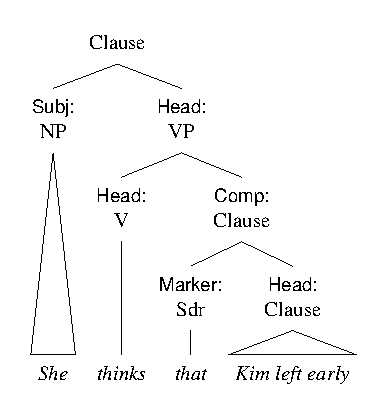
\includegraphics[width=0.55\linewidth]{figures/she thinks that kim left.pdf}
    \caption{Bağımlılaştırmayı gösteren sözdizim ağacı: \mention{She thinks that Kim left early} içinde tamlayıcı olarak \mention{that Kim left early}}\label{fig:sub-tree-sub-tr}
\end{figure}

Bağımlı yapıda \mention{that}'in kendi öbeğini yansıtmadığına, yalnızca bağımlı tümcenin başlangıcını işaretlediğine dikkat edin. \term{İşaretleyici} (\term{marker}, Mk), başının daha büyük yapıyla dilbilgisel olarak nasıl ilişkili olduğunu gösteren bir bağımlı öge türüdür.

İçerik tümceleri daha büyük yapı içinde çeşitli biçimlerde iş görebilir:

\ea \label{ex:content-funcs-tr}
    \ea \gll I suspect {\ob}that he left{\cb}.\\
        ben kuşkulan-ŞİMDİ BAĞ o ayrıl-GEÇMİŞ\\
    \glt `Onun ayrıldığından kuşkulanıyorum.' [FÖ içinde]
    \ex \gll The fact {\ob}that he left{\cb} is clear.\\
        DEF olgu BAĞ o ayrıl-GEÇMİŞ olmak açık\\
    \glt `Onun ayrıldığı olgusu açıktır.' [ADÖ içinde]
    \ex \gll I'm glad {\ob}that he left{\cb}.\\
        ben memnun BAĞ o ayrıl-GEÇMİŞ\\
    \glt `Onun ayrıldığına memnunum.' [SıfÖ içinde]
    \ex \gll We can proceed provided {\ob}that he left{\cb}.\\
        biz edebilir ilerle- koşuluyla BAĞ o ayrıl-GEÇMİŞ\\
    \glt `O ayrıldıysa ilerleyebiliriz.' [EÖ içinde]
    \ex \gll Whether or not he left is unclear.\\
        BAĞ ya-da değil o ayrıl-GEÇMİŞ olmak belirsiz\\
    \glt `Ayrılıp ayrılmadığı belirsiz.' [özne]
    \ex \gll It's unclear whether or not he left.\\
        o belirsiz BAĞ ya-da değil o ayrıl-GEÇMİŞ\\
    \glt `Ayrılıp ayrılmadığı belirsiz.' [dışa taşınmış özne]
    \z
\z

Bildirim içerik tümcelerinde işaretleyici, yani \mention{that} bağımlılaştırıcısı, tümcenin işlevine göre zorunlu, isteğe bağlı ya da kabul edilemez olabilir:
\ea\label{ex:marker-need-tr}
    \ea \gll That Kim left surprised no one.\\
        BAĞ Kim ayrıl-GEÇMİŞ şaşırt-GEÇMİŞ hiç kimse\\
    \glt `Kim'in ayrılması kimseyi şaşırtmadı.' [zorunlu]
    \ex \gll I know that Kim left.\\
        ben bil-ŞİMDİ BAĞ Kim ayrıl-GEÇMİŞ\\
    \glt `Kim'in ayrıldığını biliyorum.' [isteğe bağlı]
    \ex \gll *We left before that Kim arrived.\\
        *biz ayrıl-GEÇMİŞ önce BAĞ Kim gel-GEÇMİŞ\\
    \glt `Amaçlanan anlam: Kim gelmeden önce ayrıldık. İngilizcede \mention{that} burada kullanılamaz.' [*; kabul edilemez]
\z
\z
Özne tümceleri, (\ref{ex:marker-need-tr}a)'daki gibi, her zaman işaretleyici ister. Bildirim tümceleri tamlayıcı olarak kullanıldığında çoğunlukla işaretleyiciyle de işaretleyicisiz de gelebilir; bunu (b)'de görüyoruz. Bunun başlıca istisnası, (c)'deki gibi, EÖ içinde tamlayıcı olmalarıdır.

\label{sec:sub-interrog-tr}

Soru içerik tümceleri ilginçtir çünkü sözdizim bakımından ana tümce sorularından ayrılırlar. Ana tümce temel soruları özne-yardımcı fiil ters çevrilmesiyle tanınabilir, örneğin \mention{Did she accept?}. Buna karşılık bağımlı karşılıkları soru niteliğini \mention{whether} ya da \mention{if} ile işaretler:

\ea temel sorular\label{ex:int-sub-tr}
    \ea \gll Did she accept?\\
        YARDIMCI o kabul-et\\
    \glt `Kabul etti mi?' [ana, ters çevrilmiş]
    \ex \gll I wonder {\ob}whether she accepted{\cb}.\\
        ben merak-et-ŞİMDİ BAĞ o kabul-et-GEÇMİŞ\\
    \glt `Kabul edip etmediğini merak ediyorum.' [bağımlı]
    \z
\z
\ea odaklı sorular
    \ea \gll How did we get here?\\
        nasıl YARDIMCI biz gel- buraya\\
    \glt `Buraya nasıl geldik?' [ana, ters çevrilmiş]
    \ex \gll I wonder {\ob}how we got here{\cb}.\\
        ben merak-et-ŞİMDİ nasıl biz gel-GEÇMİŞ buraya\\
    \glt `Buraya nasıl geldiğimizi merak ediyorum.' [bağımlı]
    \z
\z
Bu, İngilizce öğrenenler için zordur. Başlangıç düzeyindekiler çoğu kez hiçbir şeyi ters çevirmez ve ana tümce sorularını yanlış kurar. Daha deneyimli öğrenciler ise ters çevirmeyi çözmüş oldukları için bunu her yerde uygular ve bağımlı soru tümcelerini yanlış yapılandırır. Öğrenciler bu ayrımı ancak oldukça ileri düzeylerde rahatça yapmaya başlar.

Ana ve bağımlı soru tümceleri arasındaki bu yapısal fark yine de çözülmeye başlamıştır; ters çevirme yavaş genişlemesini sürdürüyor. Yazıda ters çevrilmiş soru içerik tümceleri hâlâ seyrek olsa da (\ref{ex:non-inverted-interrogative-tr}) gibi örnekler konuşmada epey yaygınlaştı. Birkaç yüzyıl içinde ters çevirme bütün sorular için norm olabilir ve işaretleyiciler isteğe bağlı hâle gelebilir. Ben yine de beklemezdim.

\ea\label{ex:non-inverted-interrogative-tr}
\gll We need a story of {\ob}how did we get here{\cb}.\\
    biz gerek-duy-ŞİMDİ bir hikaye -IN nasıl YARDIMCI biz gel- buraya\\
\glt `Buraya nasıl geldik, bunun bir hikayesine ihtiyacımız var.'
\z
Şimdilik, temel soru içerik tümcelerinde bir işaretleyici, genellikle \mention{whether} ya da \mention{if}, her zaman zorunludur. Yoksa çoğu durumda bunları işaretlenmemiş bildirim tümcelerinden ayırt etmek imkansız olurdu.

\subsubsection*{Buyurucu yapı}

Bağımlı yapıların özel bir alt türü \term{buyurucu} yapıdır (\term{mandative}). Bu yapı, gereklilik ya da zorunluluk ifade eden yüklemlerle görülür:

\ea \label{ex:mandative-tr}
    \ea \gll It is essential {\ob}that he be there{\cb}.\\
        o olmak gerekli BAĞ o olmak-PLAIN orada\\
    \glt `Orada bulunması zorunludur.' [subjunctive]
    \ex \gll It is essential {\ob}that he should be there{\cb}.\\
        o olmak gerekli BAĞ o should olmak orada\\
    \glt `Orada bulunması gerekir.' [should]
    \ex \gll It is essential {\ob}that he is there{\cb}.\\
        o olmak gerekli BAĞ o olmak-ŞİMDİ orada\\
    \glt `Orada olması önemlidir.' [indicative]
    \z
\z
\term{subjunctive} varyantı fiilin yalın biçimini kullanır. \mention{should} varyantı ise Britanya İngilizcesinde daha yaygın olmuştur, en azından eskiden böyleydi. Amerikan İngilizcesi çoğu kez subjunctive yapıyı tercih eder. \term{Indicative} varyantı olağan zaman çekimli biçimi kullanır.

Bu, bağımlı tümcelerdeki çeşitlenmenin ince anlam farkları taşıyabileceğini ve bölgesel tercihleri gösterebileceğini anlatan iyi bir örnektir. Öğretim açısından, indicative biçimin özellikle gayriresmi bağlamlarda daha yaygın hâle geldiğini, ama subjunctive yapının resmi yazıda hâlâ standart olduğunu belirtmek yararlıdır.

\begin{tblsframedsymbol}{Anladığınızı kontrol edin: matris ve bağımlı}{test}
Yapısal ilişkileri belirleme alıştırması:
\begin{itemize}[noitemsep, leftmargin=*]
    \item \mention{I know that she thinks that he left} içinde ana tümceyi, matris tümceleri ve bağımlı tümceleri belirleyin.
    \item \mention{She asked whether he left} cümlesinde neden ters çevirme olmadığını, ama \mention{Did he leave?} sorusunda neden olduğunu açıklayın.
    \item Buyurucu yapıyı bulun: \mention{It's important that he be careful} ile \mention{It's important that he is careful}.
\end{itemize}
Bu yapısal ilişkileri anlamak, anlamın sözdizimsel mimariden nasıl doğduğunu açıklığa kavuşturur.
\end{tblsframedsymbol}

\subsection{Karşılaştırma tümceleri}

Sonlu bağımlı tümcelerin ikinci büyük türü karşılaştırma tümcesidir. Bunlar, (\ref{ex:comparative-intro-tr})'daki gibi, bir karşılaştırmayı tamamlayan tümcelerdir.

\ea \label{ex:comparative-intro-tr}
    \ea \gll The ice was thicker than {\ob}we expected{\cb}.\\
        DEF buz idi daha-kalın -DEN biz bekle-GEÇMİŞ\\
    \glt `Buz beklediğimizden daha kalındı.'
    \ex \gll She writes faster than {\ob}she speaks{\cb}.\\
        o yaz-ŞİMDİ daha-hızlı -DEN o konuş-ŞİMDİ\\
    \glt `Konuştuğundan daha hızlı yazar.'
    \ex \gll It doesn't cost as much as {\ob}I'd thought{\cb}.\\
        o NEG tut-DEĞER bu kadar gibi ben-düşün-GEÇMİŞ\\
    \glt `Düşündüğüm kadar pahalı değil.'
    \z
\z
Karşılaştırma tümcelerini içerik tümcelerinden ayıran şey, bağlamdan geri kazanılabilen bazı ögeleri dışarıda bırakan eksiltidir. Bunu (\ref{ex:comparative-ellipsis-tr})'deki \dots işaretlerinin gösterdiği eksiltide görebilirsiniz.\footnote{Önceki bölümlerde boşlukları tanıtmıştım. Boşluklar ağaçlarda bulunan yapısal ögelerdir. Eksilti ise bağlamdan anlamsal olarak geri kazanılabilen, ama sözdizimsel öge olmayan malzemedir.}

\ea \label{ex:comparative-ellipsis-tr}
    \ea \gll Kim read more books than {\ob}Pat read \dots{\cb}.\\
        Kim oku-GEÇMİŞ daha-çok kitap-ÇOĞ -DEN Pat oku-GEÇMİŞ \dots\\
    \glt `Kim, Pat'in okuduğundan daha fazla kitap okudu.'
    \ex \gll Kim read more books than {\ob}Pat did \dots{\cb}.\\
        Kim oku-GEÇMİŞ daha-çok kitap-ÇOĞ -DEN Pat YARDIMCI \dots\\
    \glt `Kim, Pat'in yaptığından/okuduğundan daha fazla kitap okudu.'
    \ex \gll Kim read more books than {\ob}Pat{\cb}.\\
        Kim oku-GEÇMİŞ daha-çok kitap-ÇOĞ -DEN Pat\\
    \glt `Kim, Pat'ten daha fazla kitap okudu.'
    \z
\z

İlk iki varyant eksilti gösterir; (b)'de \mention{read} sözcüğünü yinelemek yerine FÖ artgönderimi yapan \mention{did} kullanılır. Üçüncü varyantta, yani (c)'de, \mention{Pat} tümce tamlayıcısı değil ADÖ tamlayıcısıdır. Üçü de özünde aynı anlama gelir.

Çoğu eksilti türünün tersine, karşılaştırma tümcelerinde eksiltilen bilgiyi açıkça vermek dilbilgisel değildir. Örneğin *\mention{Kim read more books than Pat read 20 books} ya da *\mention{It's not as deep as it is 20 cm wide} doğru değildir. Eksilti bu tümce türünün temel parçasıdır. Karşılaştırma tümcesinin yapısı Şekil~\ref{fig:comp-tree-tr}'de gösterilmiştir.

\begin{figure}
    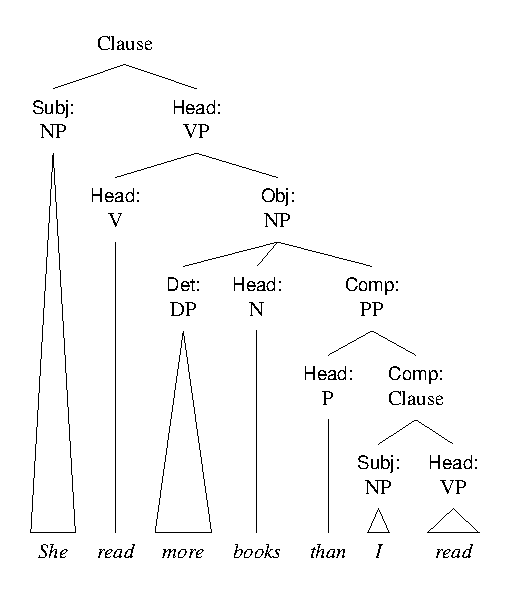
\includegraphics[width=0.7\linewidth]{figures/she read more books than I read.pdf}
    \caption{Eksiltili bir karşılaştırma tümcesini gösteren sözdizim ağacı}\label{fig:comp-tree-tr}
\end{figure}

Karşılaştırma tümceleri, yapılan karşılaştırmanın türüne göre \mention{than} ya da \mention{as} EÖ'sü içinde tamlayıcı olarak iş görür.

\ea \label{ex:comp-markers-tr}
    \ea \gll Kim is taller than {\ob}Pat is{\cb}.\\
        Kim olmak daha-uzun -DEN Pat olmak\\
    \glt `Kim, Pat'ten daha uzundur.' [eşitsizlik]
    \ex \gll Kim is as tall as {\ob}Pat is{\cb}.\\
        Kim olmak kadar uzun olarak Pat olmak\\
    \glt `Kim, Pat kadar uzundur.' [eşitlik\footnote{Buradaki \emph{eşitlik} terimi biraz yanıltıcı olabilir. Örnek, Kim'in Pat kadar, yani en az Pat kadar uzun olduğunu anlatır; Kim daha uzun da olabilir.}]
    \z
\z
(\ref{ex:comp-markers-tr}a)'daki \mention{than} eşitsizliği, (b)'deki \mention{as} ise eşitliği işaret eder. İlk \mention{as} bir zarftır: \mention{as tall} SıfÖ'sünde \mention{as} niteleyici olarak durur. İkinci \mention{as} ise edattır.

İngilizce öğrenenler için karşılaştırma tümceleri birkaç zorluk yaratır:
\begin{itemize}[noitemsep]
    \item Neyin ne zaman ve ne kadar eksiltilebileceğini anlamak.
    \item Eşitlik ve eşitsizlik örüntülerini öğrenmek.
    \item Birden fazla öge içeren karmaşık karşılaştırmalarla baş etmek.
\end{itemize}

İyi haber şu: karşılaştırma tümceleri epey düzenli örüntüler izler. Öğrenenler genellikle daha karmaşık yapılara geçmeden önce \mention{taller than} `...-den daha uzun' ve \mention{as tall as} `en az ... kadar uzun' gibi temel biçimleri öğrenebilir.

\section{Eşgüdüm}\label{sec:coordination-tr}

Bağımlılaştırma tümceler arasında bağımlılık ilişkileri kurarken, \term{eşgüdüm} eş sözdizimsel statüye sahip ögeleri birleştirir. Bu sistemin merkezinde \term{eşgüdümleyici} (\term{coordinator}, Crd) denen küçük ve kapalı bir sözcük sınıfı vardır. Başlıca üyeler \mention{and}, \mention{or} ve \mention{but}'tır. Üçünü saymak için bile üçünüze birden ihtiyaç duyarsınız. Bağımlılaştırıcılar gibi eşgüdümleyiciler de işaretleyici olarak çalışır.

Şu örnekleri düşünün:

\ea \label{ex:coord-basic-tr}
    \ea \gll {\ob}Jane is a good teacher{\cb} {\ob}and her students really like her{\cb}.\\
        Jane olmak bir iyi öğretmen ve onun öğrenci-ÇOĞ gerçekten sev-ŞİMDİ onu\\
    \glt `Jane iyi bir öğretmen ve öğrencileri onu gerçekten seviyor.'
    \ex \gll They offered us a choice of {\ob}red wine{\cb}, {\ob}white wine{\cb}, {\ob}or beer{\cb}.\\
        onlar sun-GEÇMİŞ bize bir seçenek -IN kırmızı şarap beyaz şarap ya-da bira\\
    \glt `Bize kırmızı şarap, beyaz şarap ya da bira seçeneği sundular.'
    \ex \gll Her assistant is {\ob}very young{\cb} {\ob}but a quick learner{\cb}.\\
        onun asistan olmak çok genç ama bir hızlı öğrenen\\
    \glt `Asistanı çok genç ama hızlı öğrenen biri.'
    \z
\z
Bu örneklerdeki ilgili ögeler \term{eşgüdümlü öge} (\term{coordinate}) işlevindedir. Bu işlev (\ref{ex:coord-basic-tr}a)'daki gibi tümcelerle, (b)'deki gibi ADÖ'lerle ya da başka öbeklerle, daha seyrek olarak da (c)'deki SıfÖ ve ADÖ gibi kategori karışımlarıyla gerçekleşebilir. Eşgüdümleyiciler genellikle ayrı ilişkiler ifade eder: \mention{and} ekleme, \mention{or} seçenek, \mention{but} karşıtlık bildirir.

Eşgüdümü daha önce gördüğümüz yapılardan ayıran şey başsız olmasıdır: hiçbir eşgüdümlü öge bütün yapının başı değildir. Bu başsızlık basit bir testte görünür. Çoğu durumda eşgüdümlü yapının bütününü tek tek eşgüdümlü ögelerden biriyle değiştirebilirsiniz:

\ea \label{ex:coord-replace-tr}
    \ea \gll Her assistant is very young.\\
        onun asistan olmak çok genç\\
    \glt `Asistanı çok genç.'
    \ex \gll Her assistant is a quick learner.\\
        onun asistan olmak bir hızlı öğrenen\\
    \glt `Asistanı hızlı öğrenen biri.'
    \z
\z
(\ref{ex:coord-replace-tr}a) ve (b), (\ref{ex:coord-basic-tr}c)'ye dilbilgisel alternatiflerdir. Bu durum, \mention{very young} gibi başlı yapılardan epey farklıdır. Orada başı tek başına kullanabilirsiniz, örneğin \mention{she's young}, ama bağımlıyı tek başına kullanamazsınız: *\mention{she's very}. Eşgüdüm yapısı Şekil~\ref{fig:coord-basic-tr}'de gösterilmiştir.

\begin{figure}
    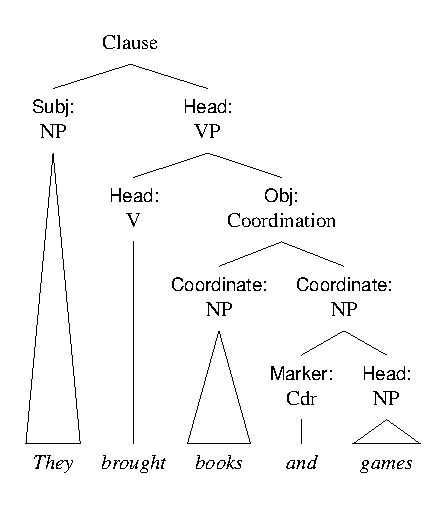
\includegraphics[width=0.65\linewidth]{figures/the brought books and games.pdf}
    \caption{İşaretleyicili temel eşgüdüm: \mention{They brought books and games}}\label{fig:coord-basic-tr}
\end{figure}

\subsection{Eşgüdümün özellikleri}

Üç temel özellik eşgüdümü başka yapılardan ayırır.

Eşgüdümlü öge sayısında dilbilgisel bir sınır yoktur. \mention{But} bunun istisnasıdır:

\ea \label{ex:coord-multiple-tr}
\gll Nothing noble, sublime, profound, delicate, tasteful or even decent can find a place.\\
    hiçbir-şey soylu yüce derin narin zevkli ya-da hatta düzgün -ebil bulmak bir yer\\
\glt `Soylu, yüce, derin, narin, zevkli hatta düzgün hiçbir şey yer bulamaz.'
\z

Eşgüdümlü ögeler işlev bakımından benzer olmalıdır: tek başlarına kullanıldıklarında aynı işlevi görebilmelidirler.

\ea \label{ex:coordinate-function-tr}
    \ea \gll I'll be back next week or at the end of the month.\\
        ben-GELECEK olmak geri gelecek hafta ya-da -DE DEF son -IN DEF ay\\
    \glt `Gelecek hafta ya da ay sonunda döneceğim.' [zaman eklentileri]
    \ex \gll *We're leaving Rome and next week.\\
        *biz-ŞİMDİ ayrıl- Roma ve gelecek hafta\\
    \glt `Amaçlanan yapı İngilizcede bozuk: \mention{Rome} nesne, \mention{next week} ise eklentidir.' [*; nesne ve eklenti]
    \z
\z

Genişletilmiş bir eşgüdümlü öge, yani eşgüdümleyicisiyle birlikte gelen öge, başa taşınamaz:

\ea \label{ex:coord-front-tr}
    \ea \gll They attended but they aren't members.\\
        onlar katıl-GEÇMİŞ ama onlar NEG-olmak üye-ÇOĞ\\
    \glt `Katıldılar ama üye değiller.'
    \ex \gll *But they aren't members, they attended.\\
        *ama onlar NEG-olmak üye-ÇOĞ onlar katıl-GEÇMİŞ\\
    \glt `Amaçlanan anlam: Katıldılar ama üye değiller. İngilizcede \mention{but} ile genişletilmiş öge böyle başa taşınamaz.' [*]
    \z
\z

\subsection{Cümle başı eşgüdümleyicilere dair bir not}

Kuralcı bir öğüt, cümleye \mention{and} ya da \mention{but} gibi eşgüdümleyicilerle başlanmaması gerektiğini söyler. Bu yasağın İngilizce dilbilgisinde ya da kullanımında temeli yoktur. Cümle başı eşgüdümleyiciler İngilizce tarihi boyunca usta yazarlarca kullanılmıştır; bu kitapta da, bu bölümde ve başka bölümlerde de pek çok örnek bulacaksınız. Cümle başındaki bir eşgüdümleyici, cümleyi önceki cümleye sıkı bir eşgüdüm içinde bağlayamaz. (\ref{ex:coord-front-tr})'deki öne taşıma kısıtını hatırlayın. Ama \term{söylem bağlayıcısı} (\term{discourse connector}) olarak iş görebilir ve yeni cümlenin öncekiyle nasıl ilişkili olduğunu gösterebilir. Tek gerçek kısıt üslupsaldır: her araç gibi cümle başı eşgüdümleyiciler de aşırı kullanıldıklarında tekdüzeleşebilir. Ölçülü kullanıldıklarında ise söylem akışını yönetmek ve metin ilişkilerini işaretlemek için değerli araçlardır.

\subsection{Eşgüdüm türleri}

En basit ayrım \term{simetrik eşgüdüm} (\term{symmetric coordination}) ve \term{asimetrik eşgüdüm} (\term{asymmetric coordination}) arasındadır. Simetrik eşgüdümde eşgüdümlü ögelerin sırası anlamı değiştirmez; asimetrik eşgüdümde değiştirir:

\ea \label{ex:coord-sym-tr}
    \ea \gll I was hungry and tired.\\
        ben idi aç ve yorgun\\
    \glt `Aç ve yorgundum.' [simetrik]
    \ex \gll I got up and had breakfast.\\
        ben kalk-GEÇMİŞ ve yap-GEÇMİŞ kahvaltı\\
    \glt `Kalktım ve kahvaltı yaptım.' [asimetrik]
    \z
\z
(\ref{ex:coord-sym-tr}a)'da eşgüdümlü ögelerin sırasını tersine çevirmek anlamı değiştirmez. Ama (b)'de sıra, olay dizisini ima eder: kalkma kahvaltıdan önce olmuştur.

\term{Dağıtıcı eşgüdüm} (\term{distributive coordination}) ve \term{ortak eşgüdüm} (\term{joint coordination}) arasında da ayrım yaparız:

\ea \label{ex:coord-dist-tr}
    \ea \gll Kim and Pat are fine players.\\
        Kim ve Pat olmak iyi oyuncu-ÇOĞ\\
    \glt `Kim ve Pat iyi oyunculardır.' [dağıtıcı]
    \ex \gll Kim and Pat are a good pair.\\
        Kim ve Pat olmak bir iyi çift\\
    \glt `Kim ve Pat iyi bir çifttir.' [ortak]
    \z
\z
(\ref{ex:coord-dist-tr}a)'da iyi oyuncu olma özelliği Kim ve Pat için tek tek geçerlidir. Ama (b)'de iyi bir çift olma özelliği yalnızca ikisine birlikte uygulanabilir; hiçbiri tek başına bir çift olamaz.

\subsection{Eşgüdümü işaretlemek}

Eşgüdüm birkaç yolla işaretlenebilir:
\begin{itemize}[noitemsep]
    \item Eşgüdümleyiciyle: \mention{red and blue}
    \item Hiç işaretleyici olmadan: \mention{red, white, blue}
    \item Yinelenen eşgüdümleyicilerle: \mention{red or white or blue}
    \item Karşılıklı işaretleyicilerle: \mention{both red and blue}
\end{itemize}

Eşgüdümleyiciler çoğu kez ekleme (\mention{and}), seçenek (\mention{or}) ve karşıtlık (\mention{but}) ifade eder. Ama asimetrik eşgüdümde ek anlamlar da taşıyabilirler:

\ea \label{ex:coord-meaning-tr}
    \ea \gll Pay within a week and you'll get a discount.\\
        öde içinde bir hafta ve sen-GELECEK al- bir indirim\\
    \glt `Bir hafta içinde ödersen indirim alırsın.' [koşullu]
    \ex \gll Pay within a week or you'll lose the discount.\\
        öde içinde bir hafta ya-da sen-GELECEK kaybet- DEF indirim\\
    \glt `Bir hafta içinde ödemezsen indirimi kaybedersin.' [olumsuz koşullu]
    \z
\z

\begin{tblsframedsymbol}{Örüntü tanıma: eşgüdüm mü bağımlılaştırma mı?}{test}
Bu yapıları ayırt etmek için tanılayıcı testleri uygulayın:
\begin{itemize}[noitemsep, leftmargin=*]
    \item \mention{She thinks that he left} ile \mention{She left and he stayed}: Hangisi bir tümceyi başka bir tümcenin içine yerleştiriyor, hangisi eş statülü iki tümceyi birleştiriyor?
    \item \mention{Although it rained, we went} ile \mention{It rained but we went}: Hangisi bağımlılık hiyerarşisi, hangisi eş statü gösteriyor?
    \item \mention{*But we went, it rained} ile \mention{Although it rained, we went}: Öne taşıma yapı hakkında ne gösteriyor?
\end{itemize}
Bu testler hiyerarşik yerleştirme ile eş statülü birleştirmeyi ayırmaya yardım eder.
\end{tblsframedsymbol}

Eşgüdümleyicileri de tanıttığımıza göre, İngilizcedeki başlıca sözcüksel kategorilerin neredeyse hepsiyle, yani ünlemler dışında hepsiyle, ve bunların tümcelerde üstlendiği ana sözdizimsel işlevlerle karşılaşmış olduk.

\subsection{Eşgüdümün yapısı}

Ögeleri eşgüdümlediğimizde aynı sözdizimsel işlevi paylaşmaları gerekir. Bu yüzden tamlayıcıları tamlayıcılarla, niteleyicileri niteleyicilerle eşgüdümleyebilirsiniz; ama bir tamlayıcıyla bir niteleyiciyi eşgüdümleyemezsiniz. Karşılaştırın:

\ea \label{ex:coord-function-tr}
    \ea \gll We listened {\ob}to the teacher{\cb} {\ob}and the students{\cb}.\\
        biz dinle-GEÇMİŞ -E DEF öğretmen ve DEF öğrenci-ÇOĞ\\
    \glt `Öğretmeni ve öğrencileri dinledik.' [tamlayıcılar]
    \ex \gll We listened {\ob}Monday{\cb} and {\ob}Tuesday{\cb}.\\
        biz dinle-GEÇMİŞ pazartesi ve salı\\
    \glt `Pazartesi ve salı dinledik.' [niteleyiciler]
    \ex \gll *We listened {\ob}to the teachers{\cb} and {\ob}Monday{\cb}.\\
        *biz dinle-GEÇMİŞ -E DEF öğretmen-ÇOĞ ve pazartesi\\
    \glt `Amaçlanan yapı İngilizcede bozuk: \mention{to the teachers} tamlayıcı, \mention{Monday} niteleyicidir.' [*; karışık işlevler]
    \z
\z
Eşgüdümlenen ögeler, yani \term{eşgüdümlü ögeler}, herhangi bir büyük öbek türünden gelebilir: adlar, fiiller, sıfatlar, edatlar ya da daha büyük öbekler ve tümceler. Önemli olan, daha büyük yapı içinde aynı biçimde iş görmeleridir.

\subsection{İşaretleyicili ve işaretleyicisiz eşgüdüm}

Eşgüdüm açık bir eşgüdümleyiciyle ya da onsuz kurulabilir. Eşgüdümleyici yoksa buna \term{bağlaçsız eşgüdüm} (\term{asyndetic coordination}) deriz:

\ea \label{ex:coord-marking-tr}
    \ea \gll She brought {\ob}games{\cb}, {\ob}stories{\cb}, {\ob}songs{\cb}.\\
        o getir-GEÇMİŞ oyun-ÇOĞ hikaye-ÇOĞ şarkı-ÇOĞ\\
    \glt `Oyunlar, hikayeler, şarkılar getirdi.' [asyndetic]
    \ex \gll She brought {\ob}games{\cb}, {\ob}stories{\cb}, and {\ob}songs{\cb}.\\
        o getir-GEÇMİŞ oyun-ÇOĞ hikaye-ÇOĞ ve şarkı-ÇOĞ\\
    \glt `Oyunlar, hikayeler ve şarkılar getirdi.' [syndetic]
    \z
\z
Tek bir eşgüdümleyiciyle kurulan basit eşgüdüme ek olarak, işaretleyicilerin birden çok eşgüdümlü ögeyle birlikte göründüğü \term{karşılıklı eşgüdüm} (\term{correlative coordination}) de vardır:

\ea \label{ex:coord-correlative-tr}
    \ea \gll {\ob}Both{\cb} tired {\ob}and{\cb} hungry\\
        hem yorgun hem aç\\
    \glt `Hem yorgun hem aç'
    \ex \gll {\ob}Either{\cb} now {\ob}or{\cb} never\\
        ya şimdi ya da asla\\
    \glt `Ya şimdi ya hiç'
    \ex \gll {\ob}Neither{\cb} simple {\ob}nor{\cb} easy\\
        ne basit ne de kolay\\
    \glt `Ne basit ne de kolay'
    \z
\z

\subsection{Katmanlı eşgüdüm}

Bazen eşgüdümlü ögelerin kendileri de eşgüdüm içerir. Buna katmanlı eşgüdüm diyebiliriz. Şu örneği düşünün:

\ea \label{ex:coord-layered-tr}
\gll The story was {\ob}short and sweet{\cb} but {\ob}complex and thought-provoking{\cb}.\\
    DEF hikaye idi kısa ve tatlı ama karmaşık ve düşünce-uyandırıcı\\
\glt `Hikaye kısa ve hoştu ama karmaşık ve düşündürücüydü.'
\z
Burada \mention{but} ile bağlanan iki ana eşgüdümlü öge var; ama bu ögelerin her birinin içinde \mention{and} ile kurulan kendi iç eşgüdümü bulunuyor. Bu katmanlanma, açık yapıyı korurken fikirler arasında karmaşık ilişkiler ifade etmemizi sağlar. Katmanlı yapı Şekil~\ref{fig:coord-layered-tr}'de gösterilmiştir.

\begin{figure}
    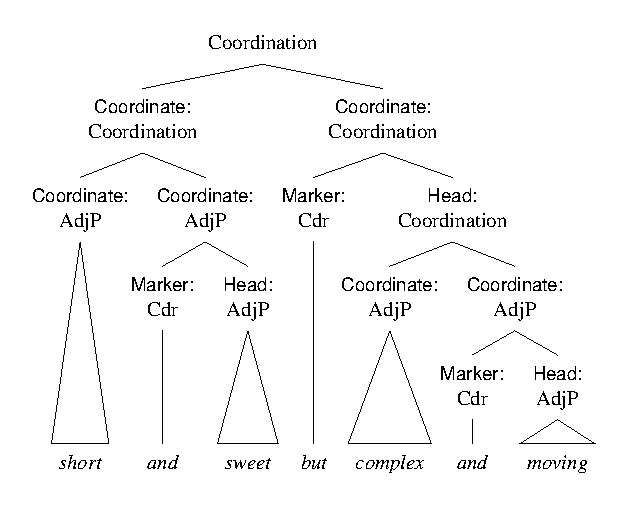
\includegraphics[width=0.9\linewidth]{figures/short and sweet but complex and moving.pdf}
    \caption{Katmanlı eşgüdüm: \mention{short and sweet but complex and moving}}\label{fig:coord-layered-tr}
\end{figure}

\subsection{Özel eşgüdüm türleri}

Özellikle ilginç bir eşgüdüm türü karşılaştırma yapılarında görülür:

\ea \label{ex:coord-comp-tr}
    \ea \gll He's as tall as {\ob}or taller than{\cb} his brother.\\
        o kadar uzun olarak ya-da daha-uzun -DEN onun erkek-kardeş\\
    \glt `Erkek kardeşi kadar uzun ya da ondan daha uzun.'
    \ex \gll She writes more {\ob}but understands less{\cb} than before.\\
        o yaz-ŞİMDİ daha-çok ama anla-ŞİMDİ daha-az -DEN önce\\
    \glt `Eskisinden daha çok yazıyor ama daha az anlıyor.'
    \z
\z
Bu yapılar çoğu kez eşgüdümlü ögeler ile paylaşılan ögeler arasında karmaşık ilişkiler içerir. Bunları yorumlamak, hem eşgüdümü hem de karşılaştırma ilişkisini anlamayı gerektirir.

\begin{tblsframedsymbol}{Hızlı öz denetim: karmaşık yapılar}{test}
Katmanlı yapıları çözümleme becerinizi sınayın:
\begin{itemize}[noitemsep, leftmargin=*]
    \item \mention{I know that she left and he stayed} içinde bütün bağımlılaştırma ve eşgüdüm ilişkilerini belirleyin.
    \item \mention{Both young and talented, she succeeded} içinde karşılıklı işaretleyicileri ve eşgüdümlü sıfatları belirleyin.
    \item Şu yapıyı çözümleyin: \mention{He's taller than I thought but shorter than his brother}.
\end{itemize}
Bu karmaşık örüntüleri anlamak, bağımlılaştırma ve eşgüdümün anlam kurmak için birlikte nasıl çalıştığını görünür kılar.
\end{tblsframedsymbol}

\section{Özet}

Bağımlılaştırma ve eşgüdüm aynı işi, yani fikirleri bağlama işini, karşıt mimarilerle yapar. Bağımlılaştırma gömer; eşgüdüm birleştirir. İyi yazı ikisini dengeler. Bir öğrencinin hangi yapıya ulaşmaya çalıştığını ve bunun nerede bozulduğunu ayırt edebildiğinizde, sorunu yalnızca sezmekle kalmazsınız. Adını koyabilirsiniz: çok fazla katman, çok fazla listeleme, ya da eşgüdümleyicinin yeterli olacağı yerde bağımlılaştırıcı kullanımı.
